\documentclass[12pt, a4paper]{article}
\usepackage{graphicx} % Required for inserting images
\usepackage[a4paper, left=4cm, right=3cm, top=3cm, bottom=3cm]{geometry}
\usepackage{indentfirst}
\usepackage{graphicx}
\usepackage{caption}
\usepackage[numbers,sort&compress]{modnatbib}
\usepackage{setspace}
\setstretch{1.5}
\usepackage{adjustbox}
%\usepackage{showframe} %use this to check if any items overlap with paper margins

%setpagenumberlocation
\usepackage{fancyhdr}
\pagestyle{fancy}
\fancyhf{} % clear the header and footer
\fancyfoot[R]{\thepage} % put the page number on the right side of the footer
\renewcommand{\headrulewidth}{0pt}

% Set fonts and spacing
\renewcommand{\familydefault}{ptm}
\setstretch{1.5}

% Set figure and table caption style
\captionsetup[figure]{font=small,labelfont={bf},labelsep=period,justification=centering}
\captionsetup[table]{font=small,labelfont={bf},labelsep=newline,justification=centering}
\usepackage{float}
\usepackage{chngcntr}
\counterwithin{table}{section}
\renewcommand{\thetable}{\thesection.\arabic{table}}
\captionsetup[table]{labelsep=space,singlelinecheck=false}
\counterwithin{figure}{section}
\renewcommand{\thefigure}{\thesection.\arabic{figure}}
\captionsetup[figure]{labelsep=space,singlelinecheck=false}

\usepackage{titlesec}

% Section style
\titleformat{\section}[display]
{\fontsize{14}{16}\selectfont\centering\normalfont\bfseries}
{SECTION \thesection}{0.1em}{\MakeUppercase}
\titlespacing*{\section}{0pt}{3.5ex plus 1ex minus .2ex}{2.3ex plus .2ex}
% Subsection style
\titleformat{\subsection}
{\normalfont\bfseries}
{\thesubsection}{12pt}{}
% Subsubsection style
\titleformat{\subsubsection}
{\normalfont\bfseries}
{\thesubsubsection}{12pt}{}

\usepackage{hyperref}
\hypersetup{colorlinks=true,linkcolor=black,citecolor=blue,urlcolor=blue}

\usepackage{lipsum}

\begin{document}

%PART1 COVER%
\pagenumbering{gobble}
\begin{center}
        \vspace*{0.5cm}
        
\includegraphics{content-headers/img-admin/pmlogo.jpg}\\
        \vspace{1cm}
        {\Large TUGAS AKHIR}\\
        \vspace{1.2cm}
        {\huge \textbf{Insert title here}\par}
        \vspace{0.8cm}
        {\Large Name \hspace{2cm} 00000000000\par}
        \vspace{9cm}
        {\textbf{PROGRAM STUDI S1 RENEWABLE ENERGY ENGINEERING}}\\
        \vspace{0.3cm}
        {\textbf{UNIVERSITAS PRASETIYA MULYA}}\\
        \vspace{0.3cm}
        {\textbf{JAKARTA, 2022}}\\
\end{center}

\newpage
\begin{center}
        \vspace*{0.5cm}
        
\includegraphics{content-headers/img-admin/pmlogo.jpg}\\
        \vspace{1cm}
        {\Large TUGAS AKHIR}\\
        \vspace{1.2cm}
        {\huge \textbf{Insert title here}\par}
        \vspace{0.8cm}
        {\Large Name \hspace{2cm} 00000000000\par}
        \vspace{1cm}
        {\textbf{TUGAS AKHIR INI DIAJUKAN UNTUK MELENGKAPI SEBAGIAN PERSYARATAN MENJADI SARJANA TEKNIK}} \par
        \vspace{7cm}
        {\textbf{PROGRAM STUDI S1 RENEWABLE ENERGY ENGINEERING}}\\
        \vspace{0.3cm}
        {\textbf{UNIVERSITAS PRASETIYA MULYA}}\\
        \vspace{0.3cm}
        {\textbf{JAKARTA, 2022}}\\
\end{center}

%PART2 ADMINDOCS%
\newpage
\pagenumbering{roman}
\setcounter{page}{2}

%%%Pernyataan keaslian tugas akhir
\section*{Halaman pernyataan keaslian tugas akhir}
\addcontentsline{toc}{section}{Pernyataan keaslian tugas akhir}
\noindent{Saya menyatakan dengan sesungguhnya bahwa tugas akhir dengan judul:
\begin{center}
    \textbf{Fabrication and Characterization of Hybrid Perovskite Solar Cell}
\end{center}
yang dibuat untuk melengkapi sebagian persyaratan menjadi Sarjana Teknik pada Pendidikan S1 Universitas Prasetiya Mulya, sejauh yang saya ketahui bukan merupakan tiruan atau duplikasi dari tugas akhir yang sudah dipublikasikan dan atau sudah pernah dipakai untuk mendapatkan gelar kesarjanaan di lingkungan Universitas Prasetiya Mulya maupun di Perguruan Tinggi atau instansi manapun, kecuali bagian yang sumber informasinya dicantumkan sebagaimana mestinya.} \par
\vspace{12cm}
\noindent Jakarta, [Insert thesis defend date here] \par
\vspace{1cm}
\noindent Tobias Haposan

%%%Pernyataan persetujuan publikasi
\newpage
\section*{Lembar pernyataan persetujuan publikasi tugas akhir untuk kepentingan akademis}
\addcontentsline{toc}{section}{Pernyataan persetujuan publikasi}
\noindent Yang bertanda tangan di bawah ini, saya mahasiswa Sekolah STEM Terapan Universitas Prasetiya Mulya: \par
\vspace{1cm}
\begin{tabular}{l l}
    Nama           & : Tobias Haposan \\
    NIM            & : 23301910001 \\
    Program Studi  & : Renewable Energy Engineering \\
\end{tabular} \vspace{1cm} \par
\noindent Demi pengembangan ilmu pengetahuan, saya memberikan Universitas Prasetiya Mulya Hak Bebas Royalti Noneksklusif (Non-exclusive Royalty Free Right) atas karya ilmiah saya baik dalam bentuk teks lengkap maupun ringkasan yang berjudul: \par
\begin{center}
    \textbf{Fabrication and Characterization of Hybrid Perovskite Solar Cell}
\end{center} \par
\noindent beserta perangkat yang diperlukan. Dengan demikian, saya memberikan hak kepada Universitas Prasetiya Mulya untuk menyimpan, mengalih media/formatkan, mengelola dalam bentuk pangkalan data, merawat, dan mempublikasikan tugas akhir saya untuk kepentingan akademis tanpa perlu meminta izin dari saya maupun memberikan royalty kepada saya selama tetap mencantumkan nama saya sebagai penulis/ pencipta dan sebagai pemilik Hak Cipta. \par
\vspace{1cm} \noindent Demikian pernyataan ini saya buat dengan sebenarnya. \par
\vspace{4cm}
\noindent Jakarta, [Insert publish date here] \par
\vspace{1cm}
\noindent Tobias Haposan

%%%Persetujuan sidang akhir
\section*{Halaman persetujuan}
\addcontentsline{toc}{section}{Persetujuan pengajuan sidang tugas akhir}
\noindent Tugas akhir dengan judul:
\begin{center}
    \textbf{Fabrication and Characterization of Hybrid Perovskite Solar Cell}
\end{center} \par
\noindent dibuat untuk melengkapi sebagian persyaratan menjadi Sarjana Teknik pada pendidikan S1 Universitas Prasetiya Mulya dan disetujui untuk diajukan dalam Sidang Tugas Akhir. \par
\vspace{15cm}
\noindent Jakarta, [Insert thesis defend date here] \par
\vspace{1cm}
\noindent \textbf{Lina Jaya Diguna} \par
\noindent Dosen Pembimbing \newpage
\section*{Acknowledgement}
\addcontentsline{toc}{section}{Acknowledgement} \newpage
\section*{Abstract}
\addcontentsline{toc}{section}{Abstract}

% Insert a table of contents
\newpage
\renewcommand\contentsname{}
\section*{Table of Contents}
\tableofcontents

\newpage
\listoffigures
\listoftables

%PART3 CONTENT%
\newpage
\setcounter{page}{1}
\pagenumbering{arabic}
\section{Introduction}
\subsection{Overview}
Recent studies of perovskite solar cells (PSCs) demonstrate that PSCs have higher experimental power conversion efficiency (PCE) when compared to silicon-based solar cells, with a record efficiency of 25.7\% as of November 2022 \cite{sharma_stability_2022, zhang_review_2022, basumatary_short_2022}. In manufacturing terms, the simplicity of large-scale fabrication such as ink-jet printing coupled with room-temperature precursor preparation conditions makes PSCs suitable for low-cost manufacturing \cite{rong_toward_2018, li_cost_2018, ahangharnejhad_impact_2022}. Unlike silicon-based solar cells, organic-inorganic PSCs can be made using solution-based precursor material. In manufacturing terms, the simplicity of utilizing solution-based precursor material for large-scale fabrication such as ink-jet printing coupled with room-temperature precursor preparation conditions makes PSCs suitable for low-cost manufacturing \cite{rong_toward_2018, li_cost_2018, ahangharnejhad_impact_2022}. The light-harvesting layer of PSCs is made from crystal perovskite with the structure of ABX\textsubscript{3}, where A is usually an organic cation, B is a metal cation, and X is a halide anion \cite{mahmud_origin_2022, correa-baena_promises_2017}. A light-harvesting layer can be prepared in the form of a liquified crystal solution. The solution can be deposited onto a substrate before being heated to form a solid thin film \cite{seok_methodologies_2018}. Solution deposition varies in techniques, some are suitable according to the cell area and material viscosity \cite{rong_toward_2018}. \par
The stability of PSCs is limited by rapid PCE degradation \cite{sharma_stability_2022, mahmud_origin_2022, seok_methodologies_2018, pean_investigating_2020, chen_synergistic_2019}. Perovskite solar cells (PSCs) are known to be unstable, which is a major challenge in developing and commercialising these devices. One source of instability is the tendency of the inorganic substances in PSCs to form hydrated products when exposed to moisture \cite{correa-baena_promises_2017, chen_synergistic_2019, cho_mixed_2018}. This can lead to rapid degradation of the power conversion efficiency (PCE) of the solar cell. One key idea for addressing this instability is to incorporate a durable organic material into the PSC to help protect it from moisture and other environmental factors. By doing so, it may be possible to improve the stability and long-term performance of PSCs \cite{seok_methodologies_2018, maafa_all-inorganic_2022}. \par
Dimensional engineering of perovskite thin film shows remarkable enhancement in both PCE and stability \cite{mahmud_origin_2022}. 2D perovskite materials are characterized by the presence of bulky organic cations, which impart several interesting properties to these materials. One property of bulky organic cations is that they are hydrophobic, which means that they do not quickly form a hydrated product when exposed to moisture, caused by the property of bulky organic cations is that they have a high barrier to ion migration, which can improve the stability of the material \cite{chen_phase_2018}. 3D perovskite materials were actually the first form of hybrid perovskite solar cells (PSCs) to be developed. One key property of 3D perovskites is that they have a lower bandgap than 2D perovskites, which means that they can absorb a wider range of wavelengths and can potentially be more efficient as light-absorbing materials. However, 3D perovskites are generally less durable than 2D perovskites when exposed to moisture and other environmental factors. In 2014, a 2D/ 3D combination showed that the respective perovskite has a slower scope of degradation and improved efficiency when combining both structures, showing it is possible to mitigate the effects of the higher bandgap by mixing 2D perovskite with conventional 3D perovskite \cite{smith_layered_2014}. According to the study, it is possible to combine both 2D and 3D perovskite materials in order to retain the desirable properties of both while omitting their weaknesses. This approach was shown to lead to an increase in power conversion efficiency (PCE) from around 2\% for 2D perovskite to 4.73\% for the hybrid material. This approach can help to improve the performance of 2D perovskite solar cells. Among the bulky organic cations, FA, MA, and PEA can be prepared and synthesized at room temperature with ambient air with relatively high stability \cite{krishna_mixed_2019, chen_stabilizing_2017, grancini_one-year_2017, cao_2d_2015, mesquita_effect_2020}. An experiment conducted by Lee et al. shows that a configuration of 3D/2D FA-MA/PEA with carbon electrode shows the highest efficiency of 14.9\% and degradation to 13.7\% after 1000 hours of operation. This experiment will attempt to replicate such a device and investigate the effect each organic has on the PSC performance.
\subsection{Problem formulation}
This experiment aims to investigate how organics affect the performance of PSC. Therefore, the goal of this experiment is to create a multidimensional hybrid perovskite solar cell and investigate the effect of the organics on performance by replicating the experiment done by Lee \textit{et al.} \cite{lee_highly_2018}. 
\subsection{Objectives}
The objective of this experiment is to fabricate hybrid 2D/ 3D perovskite solar cells (PSCs) using p-ethylenediamine (PEA), methylamine (MA), and formamidinium (FA) as organics. The resulting 2D/ 3D layers will be characterized using scanning electron microscopy and energy dispersive x-ray spectroscopy (SEM-EDX). Cell performance data will be extracted using a solar simulator, and an interaction plot will be generated to study the effect of the organics on the performance of the hybrid 2D/ 3D PSCs. This information will help to improve our understanding of the role that these organics play in the performance of hybrid 2D/ 3D PSCs and could potentially lead to the development of more efficient solar cells in the future.
\subsection{Experiment benefits}
The PSCs fabricated would then be characterized to determine their performance and efficiency, involving the measurements of their electrical properties, such as their current-voltage characteristics, and assessing their ability to convert light into electricity. The goal of the experiment would be to gain a better understanding of the organics in hybrid perovskite materials in solar cell technology and to identify any potential challenges or limitations in their use.
\subsection{Scope of experiment}
The scope of this experiment is to investigate the use of DMF:DMSO and chlorobenzene as solvents for the preparation of perovskite light harvester precursor materials, and to use PEA, MA, and FA as organic components in the fabrication of hybrid 2D/ 3D perovskite solar cells. MA and FA will be coupled to form 3D perovskite, while PEA will be used for 2D perovskite only. All annealing and sintering processes will be carried out at room temperature, and TiO\textsubscript{2} and carbon will be used as the electron transport layer (ETL) and back contact, respectively. There are several limitations to this experiment. One limitation is that only DMF:DMSO and chlorobenzene will be used as solvents for the preparation of the perovskite light harvester precursor materials, so the results may not be applicable to other solvents. Additionally, the use of only PEA, MA, and FA as organic components may not fully capture the range of possible organic compositions that could be used in the fabrication of hybrid 2D/ 3D perovskite solar cells. Finally, the fact that all annealing and sintering processes are carried out at room temperature may impact the quality and performance of the resulting solar cells.

\newpage \section{Literature review}
    \subsection{Review of studies on similar lead halide PSCs}
The combination of 2D and 3D perovskite structures has been an area of interest for researchers for some time. In addition, multiple organics have been used to create new and improved materials. These types of combinations have been previously documented and are summarized in Table 2.1. Lead halide perovskite compounds have garnered significant research attention due to their high carrier mobility, solution processability, and excellent photovoltaic properties \cite{pool_thermal_2017,sewvandi_antiferroelectric_2016,wang_surface_2017}. In carbon-based HTM-free perovskite solar cells, a carbon-based material can be used as the hole-transporting layer (HTL), which helps to transport the positive charge carriers (holes) generated by the absorption of light in the perovskite layer to the electrodes. This type of solar cell is considered "HTM-free" because it does not use a traditional hole-transporting material, such as spiro-OMeTAD or PTAA, which are commonly used in other perovskite solar cells \cite{tumen-ulzii_mini-review_2021,hawash_recent_2018,shariatinia_recent_2020}. The use of a carbon-based HTL in these solar cells has been shown to improve their performance and stability \cite{pean_investigating_2020,lee_highly_2018,maniarasu_recent_2018}.
\begin{table}[htb]
\caption{Summary of past experiments on similar PSCs.}
\begin{adjustbox}{max width=1\textwidth,center}
\begin{tabular}{c c c c}
\hline
    \textbf{Perovskite material} & \textbf{Architecture} & \textbf{PCE (\%)} & \textbf{Ref}\\ \hline
    (PEA)\textsubscript{2}(MA)\textsubscript{2}Pb\textsubscript{3}I\textsubscript{10}           & FTO/c-TiO\textsubscript{2}/perovskite/spiro-OMeTAD/Au  & 4.73  & {\cite{smith_layered_2014}} \\ \hline
    (BA)\textsubscript{2}(MA)\textsubscript{2}Pb\textsubscript{2}I\textsubscript{2}            & FTO/mp-TiO\textsubscript{2}/perovskite/spiro-OMeTAD/Au & 4.02  & {\cite{cao_2d_2015}} \\ \hline
    (BA)\textsubscript{2}(MA)\textsubscript{3}Pb\textsubscript{4}I\textsubscript{13}            & FTO/mp-TiO\textsubscript{2}/perovskite/spiro-OMeTAD/Au & 2.39  & {\cite{cao_2d_2015}} \\ \hline
    (IC\textsubscript{2}H\textsubscript{4}NH\textsubscript{3})\textsubscript{2}(MA)\textsubscript{n–1}Pb\textsubscript{n}I\textsubscript{3n+1}  & FTO/mp-TiO\textsubscript{2}/perovskite/spiro-OMeTAD/Au & 9.03  & {\cite{koh_nanostructuring_2016}}\\ \hline
    (AVA)\textsubscript{x}(MA)\textsubscript{1−x}PbI\textsubscript{3}           & FTO/mp-TiO\textsubscript{2}/mp-ZrO\textsubscript{2}/perovskite/carbon  & 11.86 & {\cite{saparov_organicinorganic_2016}}\\ \hline
    (PEA)\textsubscript{2}(MA)\textsubscript{49}Pb\textsubscript{50}Br\textsubscript{151}       & FTO/mp-TiO\textsubscript{2}/perovskite/spiro-OMeTAD/Au & 8.5   & {\cite{cohen_high_2017-1}} \\ \hline
    (PPA)\textsubscript{2}(MA)\textsubscript{49}Pb\textsubscript{50}Br\textsubscript{151}       & FTO/mp-TiO\textsubscript{2}/perovskite/spiro-OMeTAD/Au & 7.1   & {\cite{cohen_high_2017}} \\ \hline
    (BZA)\textsubscript{2}(MA)\textsubscript{49}Pb\textsubscript{50}Br\textsubscript{151}       & FTO/mp-TiO\textsubscript{2}/perovskite/spiro-OMeTAD/Au & 9.5   & {\cite{cohen_high_2017} \\ \hline
    (EDA)(MA)\textsubscript{2}{[Pb\textsubscript{3}I\textsubscript{10}]}      & FTO/mp-TiO\textsubscript{2}/perovskite/spiro-OMeTAD/Au & 11.58 & {\cite{jiang_new_2016} \\ \hline
    GAMA\textsubscript{3}Pb\textsubscript{3}I\textsubscript{10}                 & FTO/PEDOT:PSS/perovskite/PCBM/Al       & 7.26  & {\cite{soe_new_2017}} \\ \hline
    (PEI)\textsubscript{2}(MA)\textsubscript{6}Pb\textsubscript{7}I\textsubscript{22}           & ITO/PEDOT:PSS/perovskite/PCBM/LiF/Ag   & 9.39  & {\cite{yao_multilayered_2016}} \\ \hline
    (BA)\textsubscript{2}(MA)\textsubscript{3}Pb\textsubscript{4}I\textsubscript{13}   (HC)     & FTO/PEDOT:PSS/perovskite/PCBM/Al       & 12.51 & {\cite{tsai_high-efficiency_2016}} \\ \hline
    (iso-BA)\textsubscript{2}(MA)\textsubscript{3}Pb\textsubscript{4}I\textsubscript{13}   (HC) & ITO/C\textsubscript{60}/perovskite/spiro-OMeTAD/Au     & 10.63 & {\cite{chen_tailoring_2017}} \\ \hline
    (BA)\textsubscript{2}(MA)\textsubscript{3}Sn\textsubscript{4}I\textsubscript{13}            & FTO/m-TiO\textsubscript{2}/perovskite/PTAA:TPFB/Au      & 2.53  & {\cite{cao_thin_2017}} \\ \hline
    PEA\textsubscript{2}FA\textsubscript{8}Sn\textsubscript{9}I\textsubscript{28}               & ITO/NiO\textsubscript{x}/perovskite/PCBM/Al            & 5.94  & {\cite{liao_highly_2017}} \\ \hline
    (PEA)\textsubscript{2}(FA)\textsubscript{n−1}Sn\textsubscript{n}I\textsubscript{3n+1}       & ITO/PEDOT:PSS/perovskite/C\textsubscript{60}/BCP/Al    & 9.0   & {\cite{shao_highly_2018}} \\ \hline
\end{tabular}
\end{adjustbox}
\end{table}
\par \subsection{2D and 3D perovskite light harvester characteristics}
The 2D perovskite layer consists of an organic layer sandwiched with an inorganic layer \cite{krishna_mixed_2019}. The bulky organic cation is hydrophobic and has a high barrier to ion migration, meaning it will react with moisture much more slowly. But this crystal toughness results in a higher bandgap and thus less efficiency. A hybrid organic-inorganic (PEA)\textsubscript{2}(MA)\textsubscript{2}[Pb\textsubscript{3}I\textsubscript{10}] ((PEA)\textsubscript{2}(MA)\textsubscript{n−1}[Pb\textsubscript{n}I\textsubscript{3n+1}]-based PSC has the requires 2.1 eV of photon energy to produce an exciton, while a 3D equivalent made from (PEA)\textsubscript{2}(MA)\textsubscript{2}[Pb\textsubscript{3}I\textsubscript{10}]-based light harvester requires 1.63 eV. On the contrary, the 3D perovskite layer offers higher efficiency with less toughness \cite{mahmud_origin_2022}. Combining 2D with 3D perovskite layer can increase the efficiency while reducing It was introduced by Smith et al. in 2014 to increase the durability of organic-inorganic PSCs \cite{smith_layered_2014}. The idea is to combine the advantages of both structures to make a light harvester that has a lower bandgap, higher efficiency, and higher stability. A review conducted by Krishna et al. and Mahmud et al. concluded that 2D-3D perovskite light harvester performs favourably in terms of PCE parameters and stability \cite{krishna_mixed_2019,mahmud_origin_2022}.
\par \subsection{Device structure}
PSCs are configured in such a way as to maximize power conversion. Solar cells worked on the principle of the photoelectric effect, making the light-harvesting layer the core component of solar cells. Light absorption occurs within the light-harvesting layer, where an electron when excited becomes an electron-hole pair.
The device architecture of a perovskite solar cell typically consists of several layers of materials that are arranged in a specific way to allow the cell to efficiently convert sunlight into electricity. The exact composition of these layers can vary depending on the specific type of perovskite solar cell, but typically they include the following a transparent conductive layer on the front of the cell or front contact, which allows sunlight to pass through and also acts as an electrical conductor, a layer of perovskite material, which absorbs sunlight and generates charge carriers (electrons and holes) as a result, a layer of electron-transport material (ETM), which helps to collect and transport the electrons generated by the perovskite layer, a layer of hole-transport material (HTM), which allows to collect and transport the holes generated by the perovskite layer, a layer of metal on the back of the cell or back contact, which acts as a conductor and helps to collect the charge carriers generated by the perovskite layer. The structure is illustrated in Figure 2.1.
\begin{figure}[H]
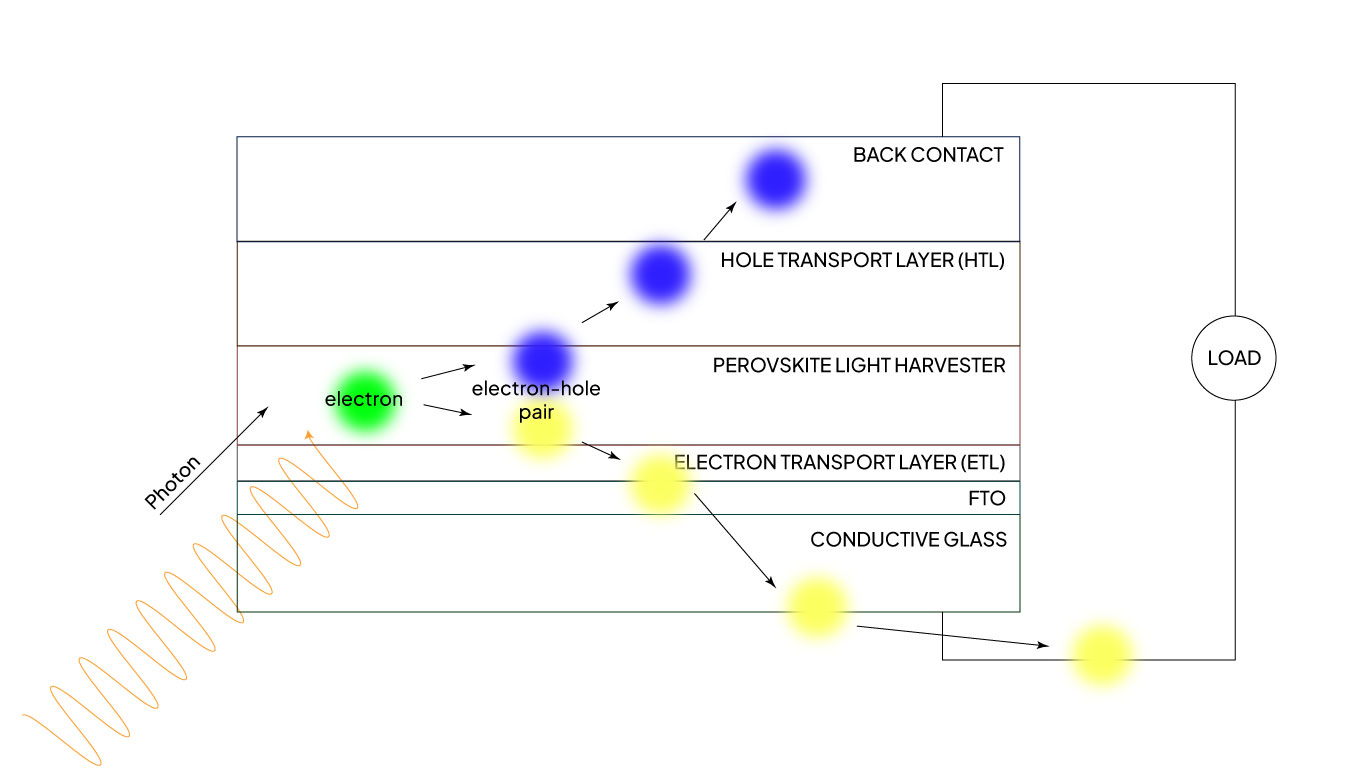
\includegraphics[width=14 cm]{img-content/psc-mechanism2.jpg}
\caption{Structure of a perovskite solar cell. Both glass (conductive) and Fluorine Tin Oxide (FTO) coats can also be collectively called front contact. A wire connecting back and front contact can be placed to allow the electron to flow\label{fig1}}
\end{figure}


\newpage \section{Methodology}
\input{content-par/03-methodology}

\newpage \section{Discussion}
\input{content-par/04-discussion}

\newpage \section{Conclusion}
\input{content-par/05-conclusion}

\newpage
\section*{References}
\addcontentsline{toc}{section}{References}
\bibliographystyle{IEEEtranN}
\renewcommand{\refname}{}
\bibliography{references}

\end{document}